In this section, the approach is evaluated in combination with the proposed heuristics using the Python implementation and with respect to the following research questions:

\begin{enumerate}
    \item[\textbf{Q1}] What is the impact of the join heuristics proposed in section \ref{section_executing_the_join}? % (1)
    \item[\textbf{Q2}] What is the impact of reducing the SHACL shape schemas and the simultaneous generation of SHACL schema validation results, depending on the schema topology and the knowledge graph used? % (1)
    \item[\textbf{Q3}] What is the impact of the parallel node plot generation as mentioned in section \ref{section_parallel_computation}?  % (2)
    \item[\textbf{Q4}] How does the decision tree visualization implementation perform in comparison to dtreeviz? % (2)
    \item[\textbf{Q5}] How much is the overhead added by the validation engine and the visualization of the annotated decision tree compared to the time needed to train the model and other interpretability methods (e.g., LIME \cite{ribeiro2016should})? % (3)
\end{enumerate}

The experimental settings are as follows:
\paragraph{Benchmarks} There are four different benchmarks used during the experimental evaluation. The first two use synthetic data to allow for load tests and the construction of benchmarks suitable to show the effect of the heuristics proposed. The latter two are benchmarks as performed in \cite{interpretME} to show two more realistic applications.

\begin{figure}
    \centering
    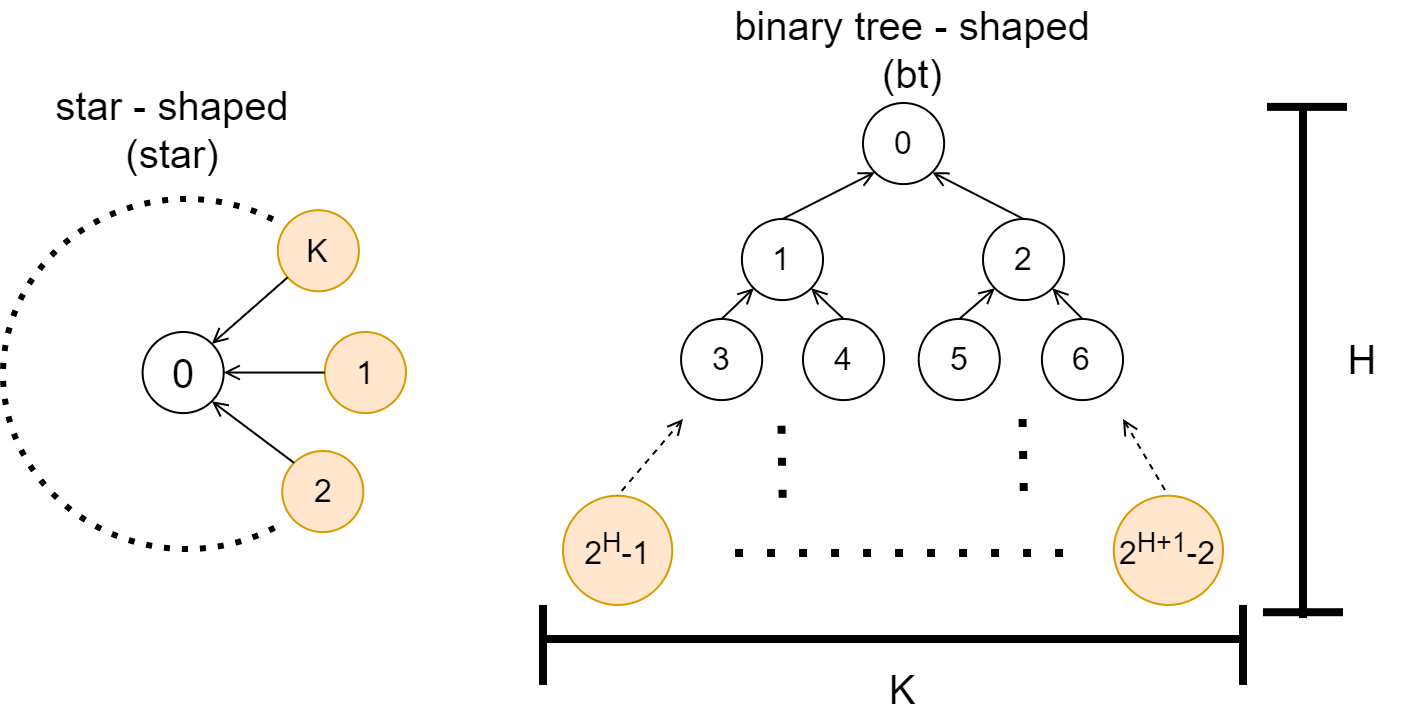
\includegraphics[width=0.8\textwidth]{images/evaluation/shape_schemes_eval.png}
    \caption{\textbf{Shape Schema Topologies of \textit{Synthetic Data A}}: $K$ denotes the number of constraints, $H$ the height of the binary tree. The nodes represent the shapes, and a directed edge connecting shape $i$ with shape $j$ represents an inter-shape constraint $(\geq_1 \uri{:link\_ij}.j)$. There are no intra-shape constraints, except shape $0$ enforces the intra-shape constraints $(\geq_l \uri{:literal\_k}.\top) \land \neg(\geq_{(m + 1)} \uri{:literal\_k}.\top)$ for all $(k,l,m) \in \{(1,1,2),(2,2,4),(3,1,8),(4,2,16)\}$.
    The $K$ colored nodes will be used as target shapes for data constraints.}
    \label{fig:shape_schemes_eval}
\end{figure}

\begin{figure}
    \centering
    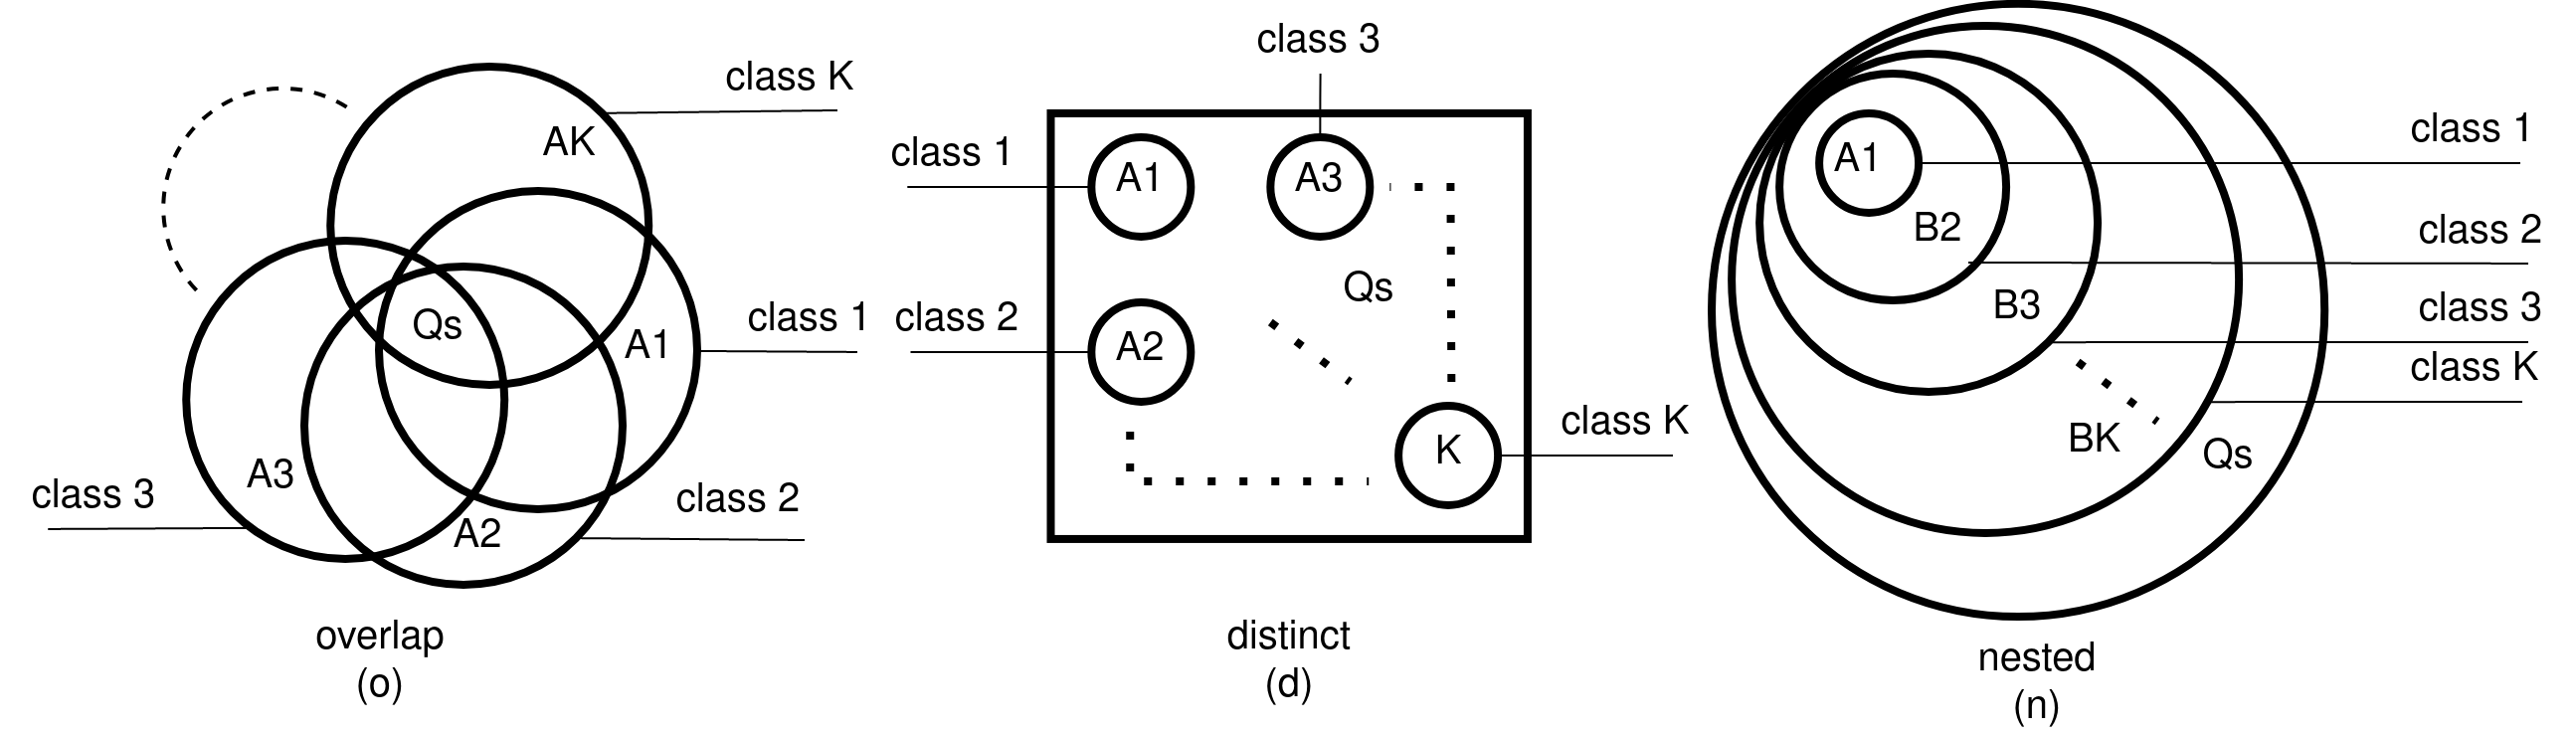
\includegraphics[width=0.8\textwidth]{images/evaluation/classes_eval.png}
    \caption{\textbf{Venn Diagrams of Classes in \textit{Synthetic Data A}}: $Qs$ is the set of entities, which will be retrieved by the seed query in the benchmarks building on \textit{Synthetic Data A}. $K$ denotes the number of constraints. Each set starting with A contains $4,000$ entities, and each set starting with B contains $4,000$ + (\#numberOfBSetsContained + 1) * $2,000$ entities. Each class not included in the figure contains $4,000$ entities. The diagram only shows the classes associated with a target definition of a target shape of a constraint.}
    \label{fig:class_venn_diagram_eval}
\end{figure}

\begin{description}
    \item[Synthetic Data A] consists of a knowledge graph $G$ with semantic data generated based on a distribution of entities to classes and a shape schema $\mathcal{S} = (\{0,1,2,..\}, \uri{TARG}, \uri{DEF})$ such that $[[\uri{TARG}(i)]]_G$ gives the entities of class $i$. Figure \ref{fig:shape_schemes_eval} depicts the two shape schema topologies which will be used: The first is a star-shaped one (short: star), and the second is a binary tree-shaped one (short: bt). For both shape schema topologies, three shape schemas of different sizes are generated, which are used in combination with the distribution of the entities to classes as schematically depicted in Figure \ref{fig:class_venn_diagram_eval}. The different test beds of \textit{Synthetic data A} can be identified with topology\_K\_distribution, where the topology is star or bt, distribution is in $\{o,d,n\}$, and $K$ denotes the number of constraints (each of the target shapes colored in Figure \ref{fig:shape_schemes_eval} belongs to a data constraint). 
    The knowledge graph is built such that for each $s \in S$, half of the entities in $[[\uri{TARG}(s)]]_G$ will be valid according to $s$. The generated knowledge graph $G$ only contains the entities and literals necessary to satisfy or violate the constraints, but does not include any further data which might be used to create the dataset and define a prediction task. Therefore, when running the validation engine over one of the test beds, the dataset generating query $Q_D$ only retrieves the seed nodes (e.g., the entities in $Qs$) to build the sample-to-node mapping $\eta$. However, this is enough to evaluate the validation engine with the heuristics proposed in section \ref{section_improving_approach} based on data constraints as they do not require a trained machine learning model to be evaluated.
    
    \item[Synthetic Data B] complements \textit{Synthetic Data A}, as the steps which could not be evaluated with \textit{Synthetic Data A} can be evaluated with \textit{Synthetic Data B}, i.e., the performance of the visualization algorithm. Therefore, the dataset $D$, the sample-to-node mapping $\eta$, as well as the entity validation function (see definition \ref{Def:shacl_entity_validation}) are generated synthetically on the basis of the number of samples $N$ (\#samples) of the dataset $D$, the number of seed nodes $M$ (\#nodes), and the number of constraints $|\mathcal{C}|$ (\#constraints). The algorithm used to generate $D$ is the one originally used to generate the \glqq Madelon\grqq{} dataset \cite{guyon2004result}, which is implemented in the scikit-learn library \cite{sklearn_api}. It basically creates clusters of samples with the same label. However, the clusters can overlap. The predictive task is a classification task; aiming to label each problem instance with its original cluster in the dataset. The default parameters used to generate $D$ can be found in table \ref{fig:parameters_used_to_generate_the_custom_dataset}. The samples-to-node mapping $\eta$ is generated by choosing randomly with uniform probability and replacement from a set of unique seed nodes with cardinality $M$. The validate function is populated as needed by the engine: Given a request $(v, s, G) \in (\mathbf{B} \cup \mathbf{I}) \times \mathbf{S} \times \mathbf{G}$ and a constraint $C \in \mathcal{C}$ the validation result is generated by a random process from $\{\top, \bot, \textit{None}\}$, where \textit{None} indicates that the entity validation function does not contain a validation result for the given request. The random process samples for each $C \in \mathcal{C}$ a triple $(p_1, p_2, p3)$ uniformly from $[0,1]^3$. The triple is normalized to $(\hat{p_1}, \hat{p_2}, \hat{p_3})$ such that $\sum_{i \in \{1,2,3\}} \hat{p_i} = 1$. Finally, for each request: $\top$ will be chosen with probability $\hat{p_1}$, $\bot$ with $\hat{p_2}$ and \textit{None} with $\hat{p_3}$.
    The data constraints can be generated by choosing a random shape schema directory and a target shape\footnote{Both do not have to exist as they will be only used to query the entity validation function for SHACL validation results}.
    The decision tree used in the benchmark is trained on $D$ with the default parameters provided by the scikit-learn library and with a maximal depth of $5$ unless specified otherwise. 
        
    \item[The French Royalty KG] is an extended version of the fully curated one proposed in \cite{Halliwell2021}. For each person in the knowledge graph, the class \uri{dbo:Person} is added. In addition, the different numbers of children, predecessors, and other counts are materialized. Furthermore, the KG is extended to include the rule-based derived \uri{dbo:hasSpouse} relationships from \cite{Halliwell2021}. Overall, this results in a knowledge graph with $3,430$ entities; having an average of 9.2 triples with the entity as the subject. The prediction task is to classify whether a person in the knowledge graph has a spouse and is tackled by the InterpretME pipeline (section \ref{section_interpretme}) to give a trained decision tree. 
    A data constraint is created for each logical rule proposed in \cite{Halliwell2021} to explain a \uri{dbo:hasSpouse} link. This procedure results in ten constraints used to validate the samples based on entities of type \uri{dbo:Person}. Each of the constraints is based on a separate shape schema with a single shape. Precisely, the constraints use different combinations of the \uri{dbo:hasChild}, \uri{dbo:hasParent}, and \uri{dbo:hasSpouse} links. For example, one constraint describes that two different people who have the same child should both have a spouse and another one stating, that if person A has person B as a spouse then person B also has a spouse.
    
    \item[The Lung Cancer KG] is a knowledge graph from the biomedical domain about lung cancer patients. For each lung cancer patient, the knowledge graph includes attributes of the individual such as gender, age, cancer stage, smoking habits, and biomarkers for lung cancer. There are a total of $21,340,353$ entities with each of them occurring in an average of $2.97$ triples as the subject. In this case, the prediction task is binary classification to predict whether the patient has ``ALK'' or ``other'' as biomarker.  Again, the task is tackled by the InterpretME pipeline to give a trained machine learning model. Data constraints are created on the basis of medical protocols. That is, special treatments should be prescribed in accordance with the patients' biomarker values. Precisely, four different data constraints are defined based on a medical protocol specifying that patients without the EGFR biomarker should not take the drugs Afatinib and Gefitinib. Each constraint is based on a target shape included in separate star-shaped SHACL schemas with three shapes (the topology is the star-shaped one in Figure \ref{fig:shape_schemes_eval} with $K=2$). 
\end{description}

\begin{table}
    \centering
    \begin{tabular}{p{7cm}|l}
        \toprule
        Parameter & Value\\
        \midrule
        \midrule
        number of clusters per class & $1$\\
        number of informative features & $2$ \\
        number of redundant/repeated features & $0$\\
        number of samples & $4^{10}$\\
        number of seed nodes & $4^{10}$\\
        number of constraints & 5 \\
        \bottomrule
    \end{tabular}    
    \caption{The default parameters used during the generation of test beds of \textit{Synthetic Data B}}
    \label{fig:parameters_used_to_generate_the_custom_dataset}
\end{table}

\paragraph{Engines} As mentioned in section \ref{section_portability_maintainability} the validation engine is agnostic to the SHACL engine; during the experimental evaluation Trav-SHACL \cite{figuera2021trav} is used. It is accessed through the \glqq ReducedTravshaclCommunicator\grqq{}, which makes use of the shaclAPI (Figure \ref{fig:shacl_api}); implementing the heuristics in \ref{section_shaclapi}.

\paragraph{Metrics}
The following metrics will be used during the evaluation of the experiments:
\begin{description}
\item[Number of SHACL validation results:] Given a set of constraints $\mathcal{C} \subset \mathbf{C}$ and a knowledge graph $G \in \mathbf{G}$, the number of SHACL validation results is $|\text{dom}(\text{validate})|$, where validate is the entity validation function generated by a SHACL engine during the evaluation of the constraints in $\mathcal{C}$.
\item[Execution time:] The elapsed time spent on executing an experiment or a part of it; measured using the Python library \emph{time}\footnote{\href{https://docs.python.org/3/library/time.html}{https://docs.python.org/3/library/time.html}}. Each experiment is executed five times and the average execution time, as well as the standard deviation of the execution times, are reported. 
All the experiments are executed on a machine equipped with an Intel$^\text{®}$ Core(TM) i5-6500 at 3.20 GHz and 8 GiB RAM.
\end{description}